\documentclass[conference]{IEEEtran}
% \IEEEoverridecommandlockouts
% % The preceding line is only needed to identify funding in the first footnote. If that is unneeded, please comment it out.
\usepackage{cite}
\usepackage{amsmath,amssymb,amsfonts}
\usepackage{algorithmic}
\usepackage{graphicx}
\usepackage{textcomp}
\usepackage{xcolor}
\usepackage{booktabs}
\def\BibTeX{{\rm B\kern-.05em{\sc i\kern-.025em b}\kern-.08em
    T\kern-.1667em\lower.7ex\hbox{E}\kern-.125emX}}
\begin{document}

\title{Supervised Learning Report}

\author{
\IEEEauthorblockN{Divyesh Baskaran}
\IEEEauthorblockA{CS7641: Machine Learning, Georgia Institute of Technology}
}

\maketitle

\section{Introduction}

General self-reported health status is a low-cost proxy used frequently to measure population-level health status, but it is challenging to predict using survey data due to its aggregation of a variety of underlying medical conditions into one ordinal category. In this report, General Health (\texttt{GenHlth}) from the 2015 Behavioral Risk Factor Surveillance System data is modeled as a multi-class problem with five target classes, and the performance of four families of supervised learning algorithms is measured against each other via a unified, leakage proof evaluation harness. The experiment follows the data first: exploratory analysis of the full dataset and a 20{,}000 row subset motivates the creation of a specific, falsifiable hypothesis about which classes can and cannot be separated using each algorithm family, and that hypothesis is directly tested, not merely mentioned. Each of Decision Trees, k Nearest Neighbors, Support Vector Machines using two kernels, and two independent PyTorch MLP models constrained to SGD only training are each separately tuned, evaluated once against the same test set, and then analyzed using learning curves, model complexity curves, and per class error analysis.

The primary finding is that the evaluation metric matters in determining which model is best: all six algorithms are nearly tied on Accuracy scores (range 0.421 to 0.468, maximum spread 0.024), but on Macro F1, a model which achieves high Accuracy fails catastrophically to predict the rarest class. The PyTorch MLP model achieves the best overall Macro F1 and balanced accuracy of any model evaluated, and all six models, regardless of algorithm family, struggle significantly to separate the two most serious health status categories, a trend traced back to a particular feature limitation from exploratory analysis.

\section{Exploratory Data Analysis}

\subsection{Dataset}

The data set used is the Diabetes Health Indicators Dataset derived from the 2015 Behavioral Risk Factor Surveillance System (BRFSS), specifically the file \texttt{diabetes\_012\_health\_indicators\_BRFSS2015.csv}, containing 253,680 respondent records and 22 columns. The target for prediction is \texttt{GenHlth}, which is a 5 level self reported general health rating (1=Excellent to 5=Poor), which is treated as a five class multiclass classification problem. The remaining 21 columns consists of 14 binary health indicators (e.g., \texttt{HighBP, Smoker, DiffWalk}), 2 bounded variable in the range of 0-30 of recorded poor days of mental of physical health (\texttt{MentHlth, PhysHlth}), 1 continuous variable of \texttt{BMI}, and a three level status of diabetes (\texttt{Diabetes\_012}) which is kept as a predictor separate from the target. There are no missing variables, however 23,899 rows (9.4\%) are duplicates. 

\subsection{Exploratory Data Analysis}

The target distribution of the data is unevenly weighed towards the moderate health ratings. Classes 2 and 3 (Very Good and Good respectively) account for a majority of the data (35.1\% and 29.8\% respectively). Class 5 (Poor) accounts for 4.8\% (Table 1). None of the classes goes below 1\% of the data, which makes the imbalance but not unnoticeable. A classifier attempting to optimize for raw accuracy would score deceptively well while improperly predicting class 5. This gives justification to use Macro-F1, balanced accuracy, and accuracy to show class specific behavior in the results that follow. 

\begin{table}[htbp]
\caption{Full-data class distribution}
\label{tab:full-dist}
\centering
\begin{tabular}{lrr}
\toprule
\textbf{GenHlth} & \textbf{Count} & \textbf{Share (\%)} \\
\midrule
1 (Excellent) & 45{,}299 & 17.86 \\
2 (Very Good) & 89{,}084 & 35.12 \\
3 (Good)      & 75{,}646 & 29.82 \\
4 (Fair)      & 31{,}570 & 12.44 \\
5 (Poor)      & 12{,}081 &  4.76 \\
\bottomrule
\end{tabular}
\end{table}

The duplicate rows were examined to determine if they were distributed proportionally to the target, since removing non proportionate duplicates would distort the distribution. The duplicated were concentrated in classes 1 and 2 (accounting for 40.4\% and 49.4\% of the duplicate rows, compared with 17.9\% and 35.1\% of the full data). The duplicated were rarely found in classes 4 and 5. This is consistent with healthy respondents reporting no conditions, making it possible identical rows from different people possible, rather than an error in the data collection. The analysis will include the duplicate rows, since removing them would disproportionately understate the true prevalence of the majority health cases. 

Feature scales varies across the predictor set. 14 of the 21 predictors are binay,  BMI ranges 12-98 (mean 28.4, std 6.6), and count features of \texttt{MentHlth/PhysHlth} range 0-30 and are right skewed (std\textgreater mean). This means scaling is important before kNN, SVM, and neural network models which are distance or gradient based. Decision trees do not need this scaling since they split on thresholds. 

Class conditional means (Fig. 1) reveal two separation shapes. \texttt{PhysHlth} and \texttt{DiffWalk}, the features most closely correlated with \texttt{GenHealth} (r=0.56, 0.46), are mostly flat for classes 1-3 then shoot up at classes 4-5 (mean \texttt{PhysHlth}: 0.86 → 3.39 → 11.4 → 23.5). This is a threshold like shape. \texttt{Income, Education,} and \texttt{PhysActivity} instead shift smoothly (Income falls only 6.82 → 6.58 from class 1 to 2). BMI also rises through to class 4, but is flat between classes 4 and 5, which means that this cannot separate from Fair and Poor. 

\begin{figure}[htbp]
\centering
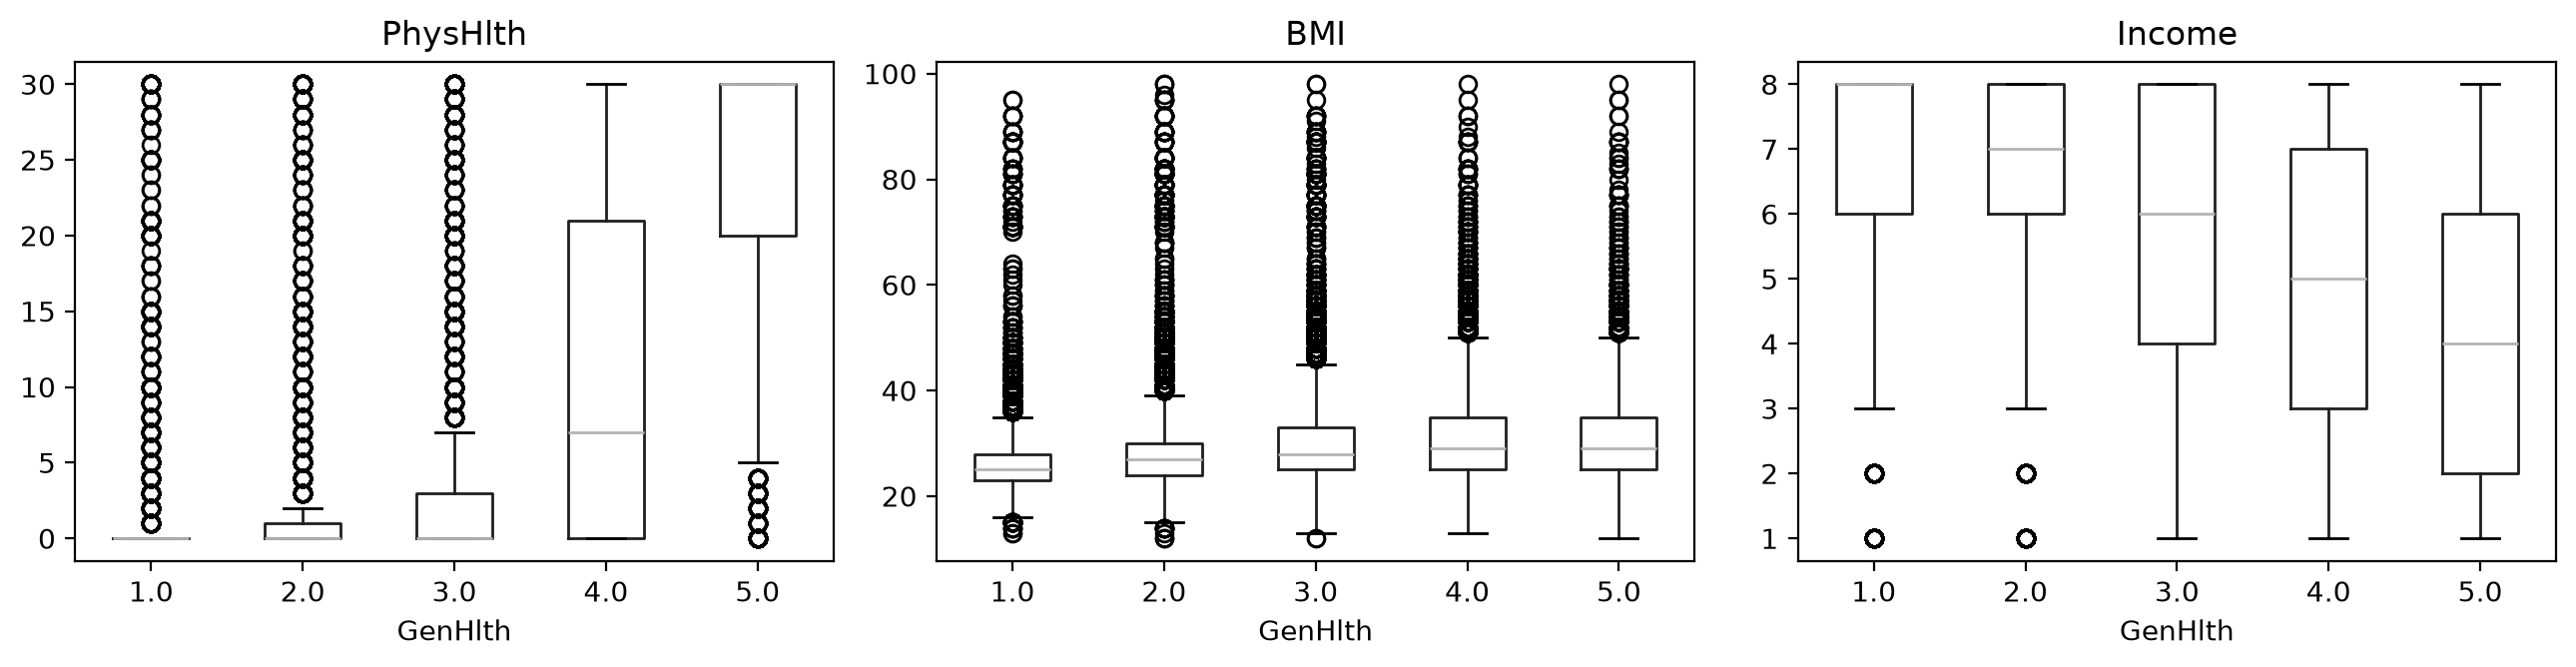
\includegraphics[width=\columnwidth]{figures/eda_class_conditional.png}
\caption{Class-conditional distributions of \texttt{PhysHlth}, \texttt{BMI}, and \texttt{Income} across \texttt{GenHlth} classes 1--5. \texttt{PhysHlth} shows a threshold-like jump at classes 4--5; \texttt{Income} shifts more smoothly with overlapping adjacent classes.}
\label{fig:class-conditional}
\end{figure}

\subsection{Sampling Design}

A stratified random sample of 20,000 rows on \texttt{GenHlth} (Seed 42) was drawn to preserve class proportions on purpose rathar by chance. The first 20,000 rows were avoided in case of ordering effects. The sample matches the full data distribution present in the full data set to within 0.01 percentage points per class (Table II, Fig.2). The largest feature mean shift is 0.037 \texttt{Age}, showing the feature relationships were preserved as well. 

\begin{table}[htbp]
\caption{Full vs.\ sampled class distribution}
\label{tab:sample-dist}
\centering
\begin{tabular}{lrrr}
\toprule
\textbf{GenHlth} & \textbf{Full (\%)} & \textbf{Sample (\%)} & \textbf{Abs.\ diff (pp)} \\
\midrule
1 & 17.86 & 17.85 & 0.01 \\
2 & 35.12 & 35.12 & 0.00 \\
3 & 29.82 & 29.82 & 0.00 \\
4 & 12.44 & 12.44 & 0.00 \\
5 &  4.76 &  4.76 & 0.00 \\
\bottomrule
\end{tabular}
\end{table}

\begin{figure}[htbp]
\centering
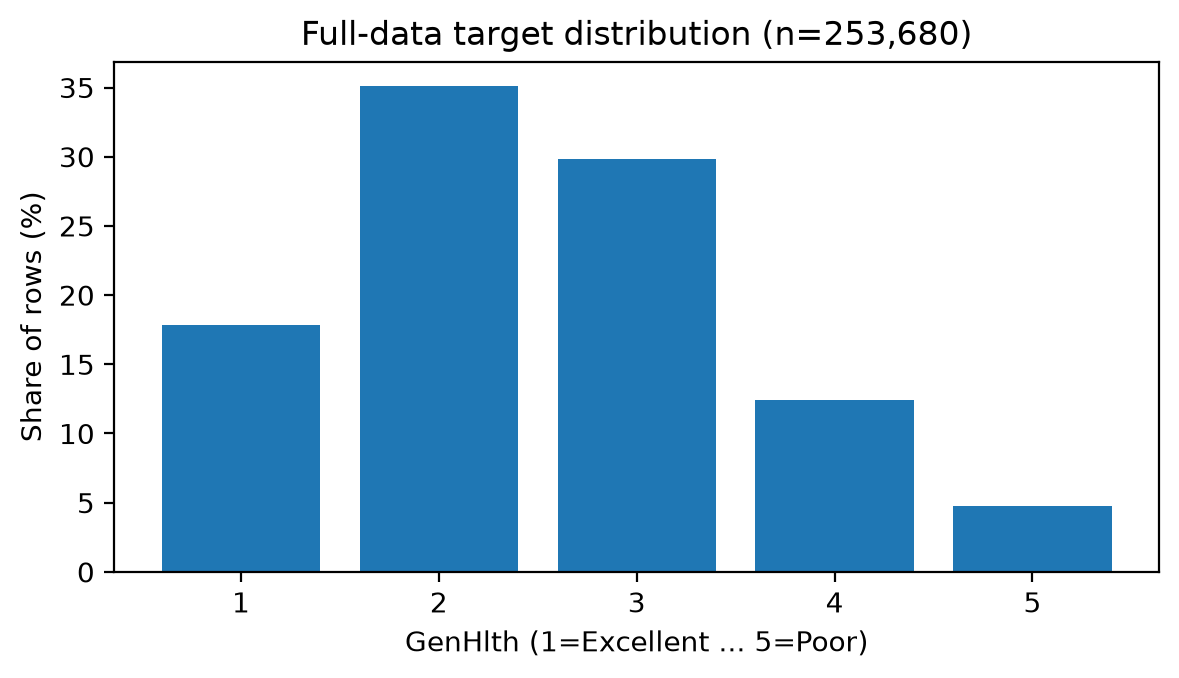
\includegraphics[width=\columnwidth]{figures/eda_class_distribution.png}
\caption{Full-data vs.\ sampled \texttt{GenHlth} class distribution ($n=253{,}680$ full, $n=20{,}000$ sample).}
\label{fig:class-dist}
\end{figure}

After an 80/20 split, the rarest class 5 has 191 test rows out of 953 total sampled rows. This is a low sample but still usable for a per class F1 estimate. 

\subsection{Hypothesis}

\textbf{Hypothesis Part 1: A pruned Decision Tree will match or outperform a linear SVM in the extreme cases (1 vs. 5).} This is due to \texttt{PhysHlth} and \texttt{DiffWalk} separate the low and high classes drastically with a sharp threshold which a decision tree can exploit directly, where a linear boundary must compromise across a range where those values barely move. 

Additionally, \textbf{Hypothesis Part 2: A RBF-kernel SVM or MLP should outperform the tree on the more difficult adjacent classes (classes 2 vs. 3 vs. 4).} This is due to the shifts happening more gradually coming from \texttt{Income, Education,} and \texttt{PhysActivity} which a single threshold cannot cleanly separate. 

Overall, I expect Decision Tree to do well in the extreme class classification and RBF SVM or MLP to do better in the moderate class ranges. 

\section{Methodology}

\subsection{Training vs. Test Split and Preprocessing}

A single split of 80/20 of the 20,000 row sample produced 16,000 training and 4,000 test rows. The test set is only touched once at final evaluation. All 21 features are standardized with a scalar fit on the training data. The decision tree is fit without this step, since its splits are invariant of monotonic scaling. 

\subsection{Tuning Protocol}

Hyperparameters are selected via 5 fold stratified cross validation on the training set, scored on Macro F1 rather than Accuracy, since Accuracy can reward settings that favor the majority classes without that trade off appearing in the score being optimized \cite{he2009}. This protocol is applied identically across all four required algorithm families, Decision Tree, kNN, SVM, and Neural Networks, the last implemented separately in scikit-learn and PyTorch, six trained model configurations in total. A single random seed (42) is used throughout for sampling, the train and test split, cross validation folds, every model's own random state, and PyTorch's initialization, so each experiment in this study is reproducible from that one value. As a check, a reference Logistic Regression's cross validated Macro F1 ($0.428 \pm 0.018$) and held out test Macro F1 (0.417) were reasonably close, providing a useful sanity check on the evaluation protocol.

\subsection{Leakage / Evaluation Debug}

Table~\ref{tab:baselines} reports two sanity baselines against the held out test set: a most frequent dummy classifier, and a Logistic Regression trained on randomly shuffled training labels. The dummy classifier reaches 0.351 accuracy but only 0.104 Macro F1 and 0.200 balanced accuracy, the numeric basis for treating Accuracy alone as insufficient. The shuffled label model collapses to nearly the same scores (0.361 / 0.128 / 0.208), the expected result when no true signal survives label shuffling. A Logistic Regression trained on the real labels clearly separates from both (0.468 / 0.417 / 0.400), confirming the harness can detect genuine signal as reliably as it fails to find one where none exists.

\begin{table}[htbp]
\caption{Sanity baselines on the held out test set}
\label{tab:baselines}
\centering
\small
\begin{tabular}{lrrr}
\toprule
\textbf{Model} & \textbf{Acc.} & \textbf{Macro F1} & \textbf{Bal. Acc.} \\
\midrule
Dummy (most frequent) & 0.351 & 0.104 & 0.200 \\
Log. Reg., shuffled labels & 0.361 & 0.128 & 0.208 \\
Log. Reg., real labels & 0.468 & 0.417 & 0.400 \\
\bottomrule
\end{tabular}
\end{table}

Every model's final evaluation returns Accuracy, Macro F1, balanced accuracy, a confusion matrix, and per class precision, recall, and F1, using one common reporting function to ensure evaluation consistency between all six models.

\subsection{Hardware and Environment}
All experiments ran on one machine with an Apple M2 Pro CPU and 16 GB of RAM. No GPU was used for either neural network. The environment used Python 3.12, scikit-learn 1.9.1, and PyTorch 2.14.0.

\section{Algorithm Results}

\subsection{Decision Tree}
An unregularized tree overfits the data severely. The cross Macro F1 is 0.351$ +-$ 0.010 versus 0.987on the training data it was fit on. This confirms printing is necessary rather than optional. \texttt{max\_depth} is used as the sole complexity control, chosen for direct interpretability. The criteria for the split is Gini impurity compared directly against entropy at depth 6, the two producted very similar cross validated scores. (Gini $0.420 \pm 0.020$ vs.\ entropy $0.423 \pm 0.019$). Gini is used for lower computational cost given the negligible difference observed. Fig. 3 shows the resulting bias variance trade off. Validation Macro F1 rises from 0.197 at depth 1 to a peak of 0.420 at depth 6, then falls to 0.350 by depth 30 as training Macro F1 keeps climbing to 0.988. The learning curve at the unpruned setting shows training Macro F1 near 1.0 and validation Macro F1 flat near 0.35 across every training size from 1,280 to 12,800 rows. The gap does not close with more data, which confirms a variance problem that only pruning can address. 

A fine grid search around the coarse optimum confirms \texttt{max\_depth=6} (CV Macro F1 0.420). Refit on the full training set and evaluated once on the held out test set, the tuned tree reaches 0.443 accuracy, 0.421 Macro F1, and 0.401 balanced accuracy, comparable to the reference Logistic Regression (0.468/0.417/0.400) despite being a much simpler model, and roughly 0.07 Macro F1 above the unpruned baseline's CV score. Fit time is 23.8~ms and predict time 2.0~ms on the 4,000 row test set, the cheapest of the six model configurations. The final tree has depth 6 and 64 leaves.

Per class recall is highest for class 2 (0.559) and lowest for classes 1 (0.319) and 5 (0.330). Errors concentrate on adjacent classes throughout, and most strikingly, 103 of class 5's 128 misclassifications (80\%) land in class 4 specifically. This pattern is consistent with the hypothesis's prediction of persistent class 4 and 5 confusion, though the experiment does not isolate \texttt{BMI}'s individual contribution from the other predictors.

\begin{figure}[htbp]
\centering
\begin{minipage}{0.49\columnwidth}
\centering
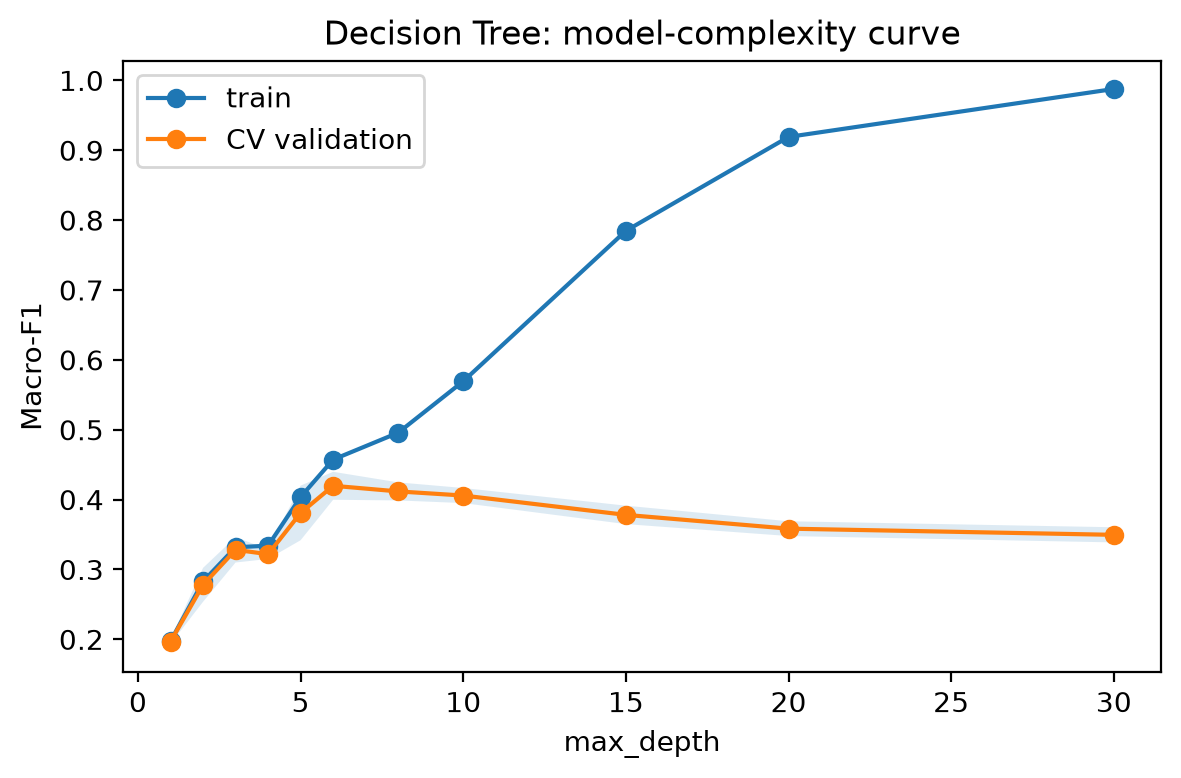
\includegraphics[width=\textwidth]{figures/dt_complexity_curve.png}
\end{minipage}
\hfill
\begin{minipage}{0.49\columnwidth}
\centering
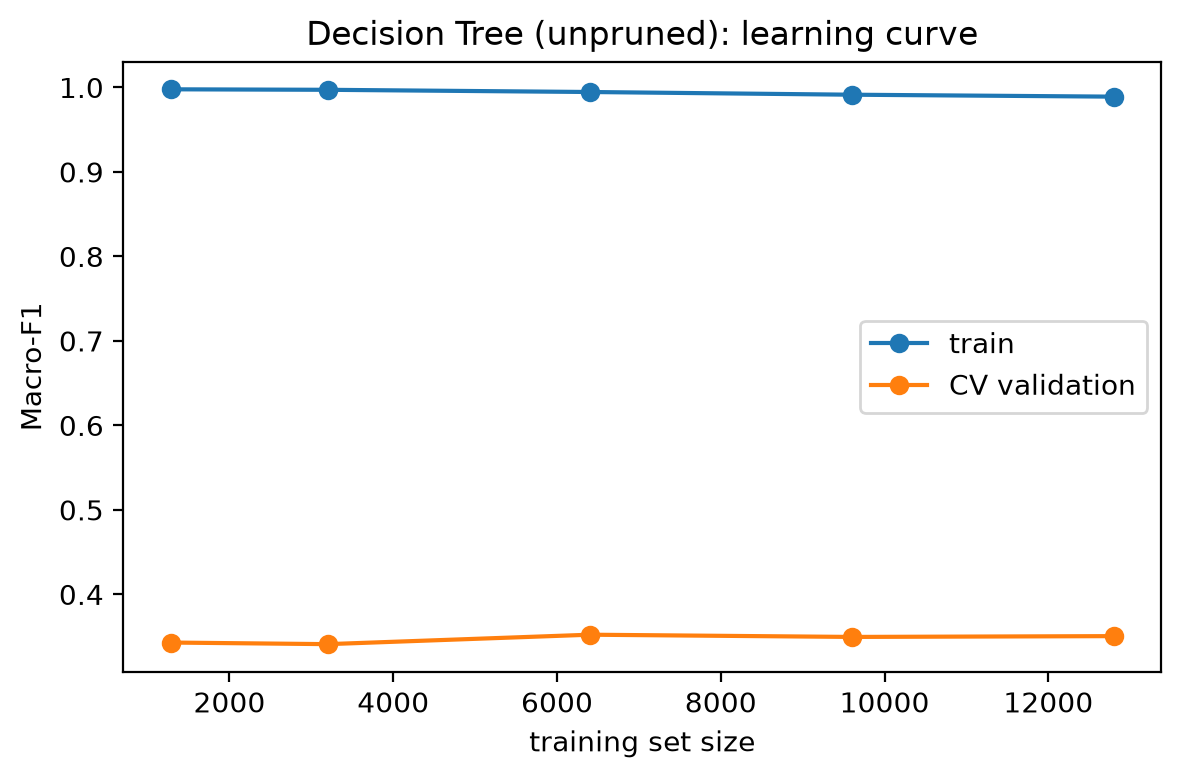
\includegraphics[width=\textwidth]{figures/dt_learning_curve.png}
\end{minipage}
\caption{Decision Tree model complexity curve (left, Macro F1 vs.\ \texttt{max\_depth}, peaking at depth 6) and learning curve at the unpruned setting (right). The train and validation gap persists across all training sizes, indicating high variance rather than insufficient data.}
\label{fig:dt-complexity}
\label{fig:dt-learning}
\end{figure}

\subsection{kNN}

Distance weighting was tested against uniform weighting at $k=11$ and found not to matter (0.386 vs.\ 0.381 CV Macro F1, within one standard deviation). We proceed with uniform weighting and Euclidean distance, the standard choice once features are scaled. A default $k=5$ already reduces the extreme memorization seen in the unpruned tree, but with room to improve: CV Macro F1 is $0.365 \pm 0.012$ against a training Macro F1 of 0.551.

Fig.~\ref{fig:knn-complexity} sweeps $k$ from 1 to 101. At $k=1$, training Macro F1 is 0.988 (pure memorization) while validation is only 0.352, the widest gap in the sweep. Validation Macro F1 peaks at 0.390 at $k=21$ before falling to 0.357 by $k=101$ as the neighborhood oversmooths toward the global class distribution. This is the same bias variance shape as the Decision Tree's complexity curve, parameterized by neighborhood size instead of depth. Notably, the learning curve at $k=5$ (Fig.~\ref{fig:knn-learning}) behaves differently from the tree's: validation Macro F1 rises from 0.331 to 0.365 as training data grows, since kNN's effective capacity depends on local sample density rather than a fixed parameter count. More data plausibly would help kNN further, unlike the Decision Tree.

\begin{figure}[htbp]
\centering
\begin{minipage}{0.49\columnwidth}
\centering
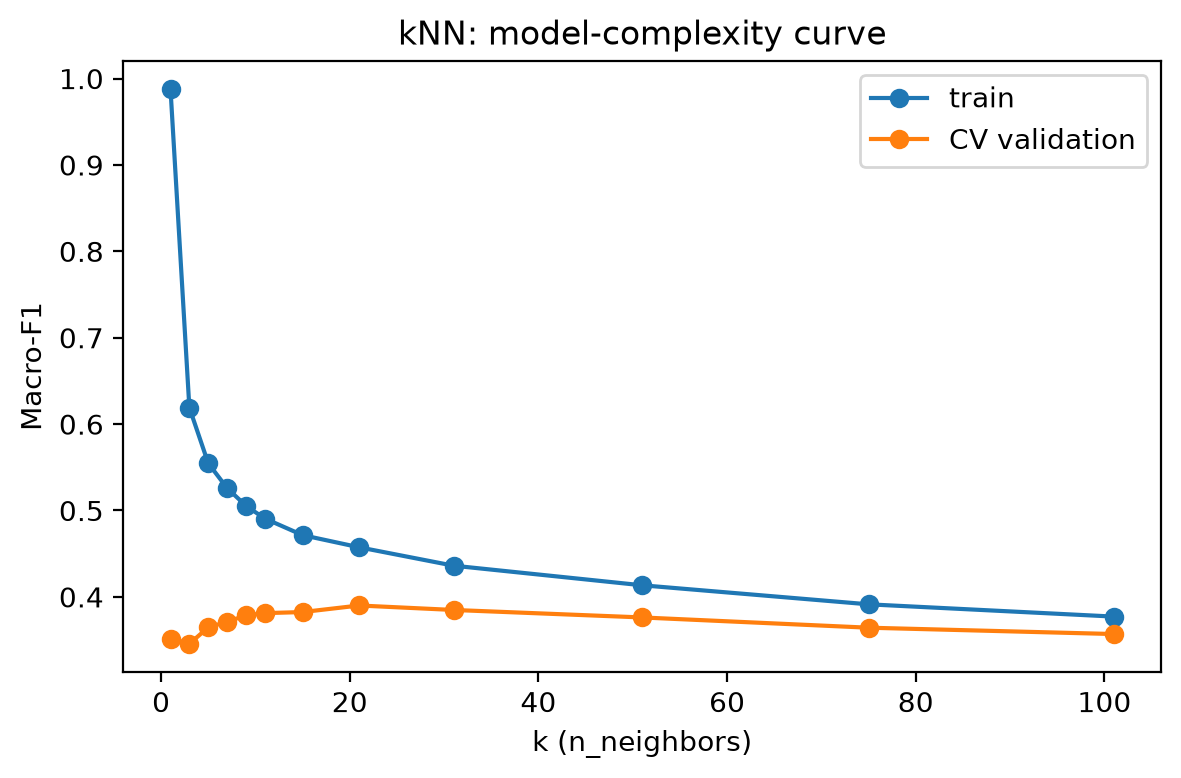
\includegraphics[width=\textwidth]{figures/knn_complexity_curve.png}
\end{minipage}
\hfill
\begin{minipage}{0.49\columnwidth}
\centering
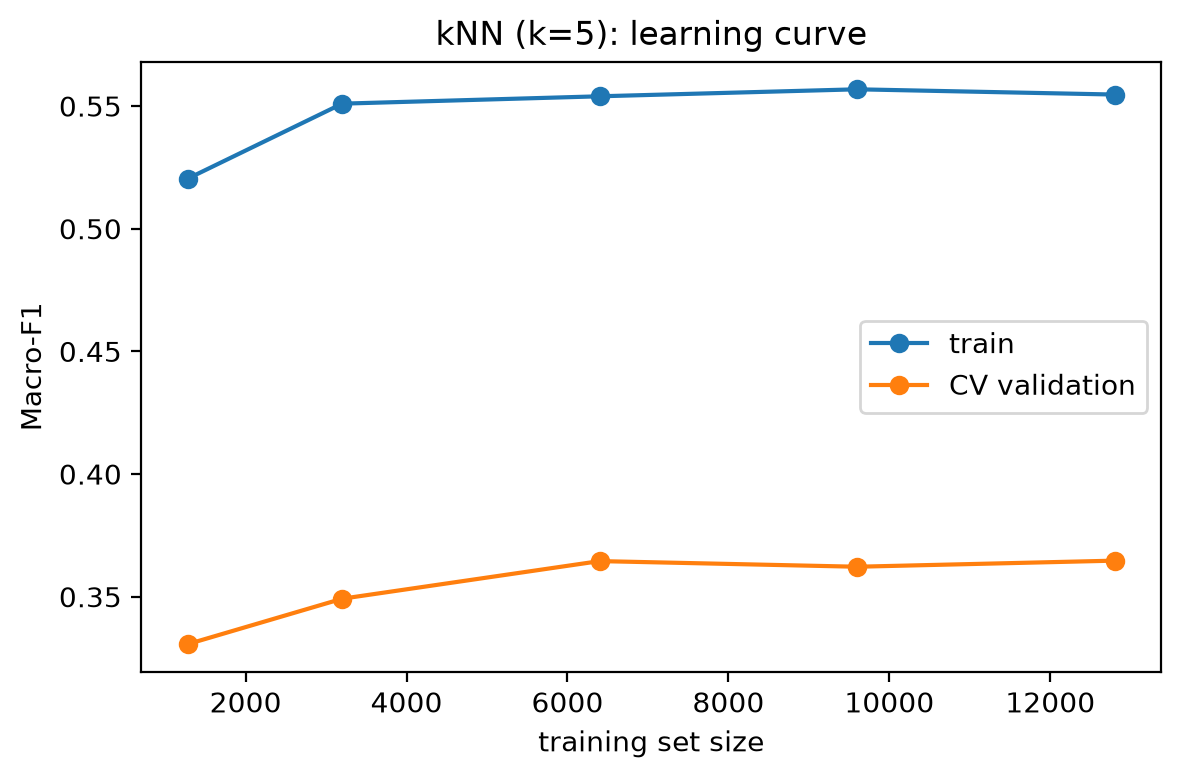
\includegraphics[width=\textwidth]{figures/knn_learning_curve.png}
\end{minipage}
\caption{kNN model complexity curve (left, Macro F1 vs.\ $k$, peaking at $k=21$) and learning curve at $k=5$ (right). Unlike the Decision Tree, validation performance improves with more training data.}
\label{fig:knn-complexity}
\label{fig:knn-learning}
\end{figure}

A fine grid search confirms $k=21$ (CV Macro F1 0.390). On the held out test set, the tuned kNN reaches 0.444 accuracy, 0.410 Macro F1, and 0.386 balanced accuracy, essentially tied with the Decision Tree on accuracy but slightly behind on Macro F1 and balanced accuracy. Fit time is 5.4~ms, but predict time is 57.6~ms on the 4,000 row test set, roughly 11x slower to predict than to fit, and about 29x slower to predict than the Decision Tree on the same test set, the expected cheap fit, expensive predict trade off for a distance based method.

Recall is highest for class 2 (0.623) and lowest for class 4 (0.279), a different weak point than the tree, which struggled most with classes 1 and 5. Errors at the class 4 and 5 boundary run in both directions (65\% of class 5's errors land in class 4, and 8\% of class 4's land in class 5), again consistent with the hypothesis's prediction that \texttt{BMI}'s plateau leaves little signal to separate these two classes regardless of algorithm family.

The feature set mixes binary indicators, bounded count variables, ordinal variables, and one continuous variable. Standardizing all of them before computing Euclidean distance still imposes a particular geometry: binary indicators contribute discrete unit sized changes while ordinal variables are treated as evenly spaced numeric scales, and every feature counts equally toward distance regardless of how much class information it carries. Because 14 of the 21 features are binary and the redundancy screen found only weak pairwise correlation among them, several binary indicators likely contribute mostly noise to each distance calculation, a plausible reason the model complexity curve needed a fairly large neighborhood ($k=21$) to dilute that noise.

\subsection{SVM}

Support Vector Machines separate classes by maximizing the margin between them, and the kernel trick allows a nonlinear decision boundary without explicitly constructing the higher dimensional mapping \cite{cortes1995}. A timing check found a single SVC fit on the full training set costs 7 to 9 seconds regardless of kernel, making full 5 fold cross validation over a hyperparameter grid impractical, so SVM tuning uses a single stratified 80/20 validation split instead, with the held out test set still touched exactly once at final evaluation. Both kernels use nearly every training point as a support vector at default settings (linear 12{,}528/12{,}800, 98\%, RBF 12{,}346/12{,}800, 96\%), consistent with the class overlap suspected from EDA.

Fig.~\ref{fig:svm-linear} shows the linear kernel's $C$ sweep: validation Macro F1 is completely flat at 0.339 from $C=0.1$ through $C=100$, a hard ceiling that more margin tightening cannot cross. Fig.~\ref{fig:svm-rbf} shows the RBF kernel's $\gamma$ sweep instead: validation Macro F1 peaks at 0.388 at $\gamma=0.1$, then collapses to 0.245 and 0.154 at $\gamma=1$ and $\gamma=10$ even as training Macro F1 keeps rising to 0.975, a severe, textbook overfitting signature as the boundary becomes increasingly local. The learning curve at a representative RBF setting (Fig.~\ref{fig:svm-learning}) is unusual: training Macro F1 falls from 0.759 to 0.625 as data grows while validation Macro F1 rises from 0.359 to 0.388, still climbing at the largest size. Unlike the Decision Tree, more data would plausibly help this model further.

\begin{figure}[htbp]
\centering
\begin{minipage}{0.49\columnwidth}
\centering
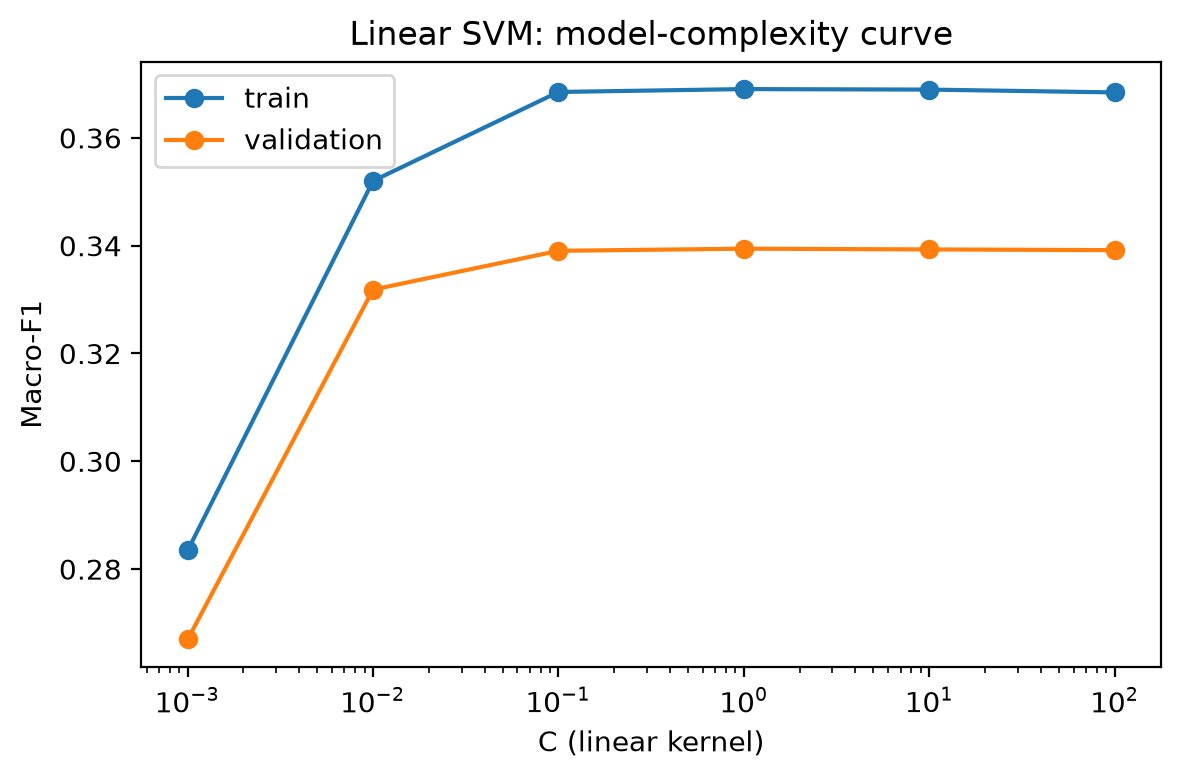
\includegraphics[width=\textwidth]{figures/svm_linear_complexity_curve.png}
\end{minipage}
\hfill
\begin{minipage}{0.49\columnwidth}
\centering
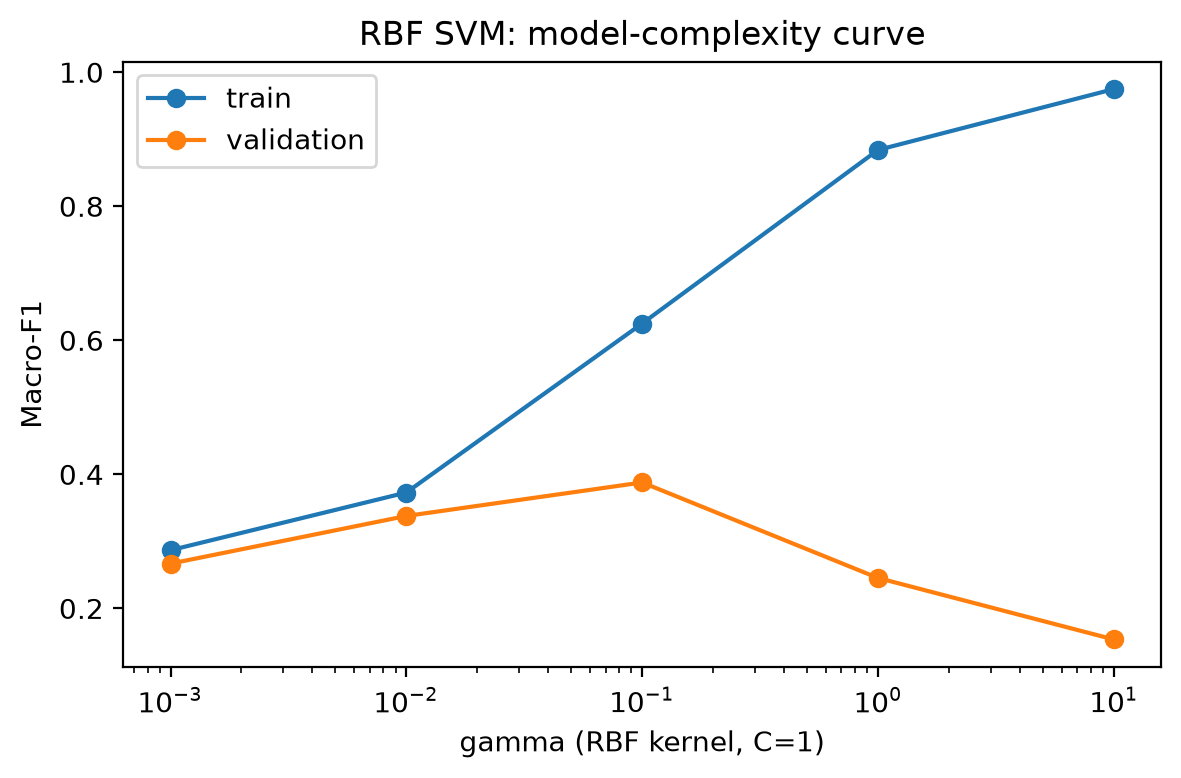
\includegraphics[width=\textwidth]{figures/svm_rbf_complexity_curve.png}
\end{minipage}
\caption{Linear SVM model complexity curve (left, Macro F1 vs.\ $C$, plateauing past $C=0.1$) and RBF SVM model complexity curve (right, Macro F1 vs.\ $\gamma$ at $C=1$, peaking at $\gamma=0.1$ then collapsing as training performance keeps rising).}
\label{fig:svm-linear}
\label{fig:svm-rbf}
\end{figure}

\begin{figure}[htbp]
\centering
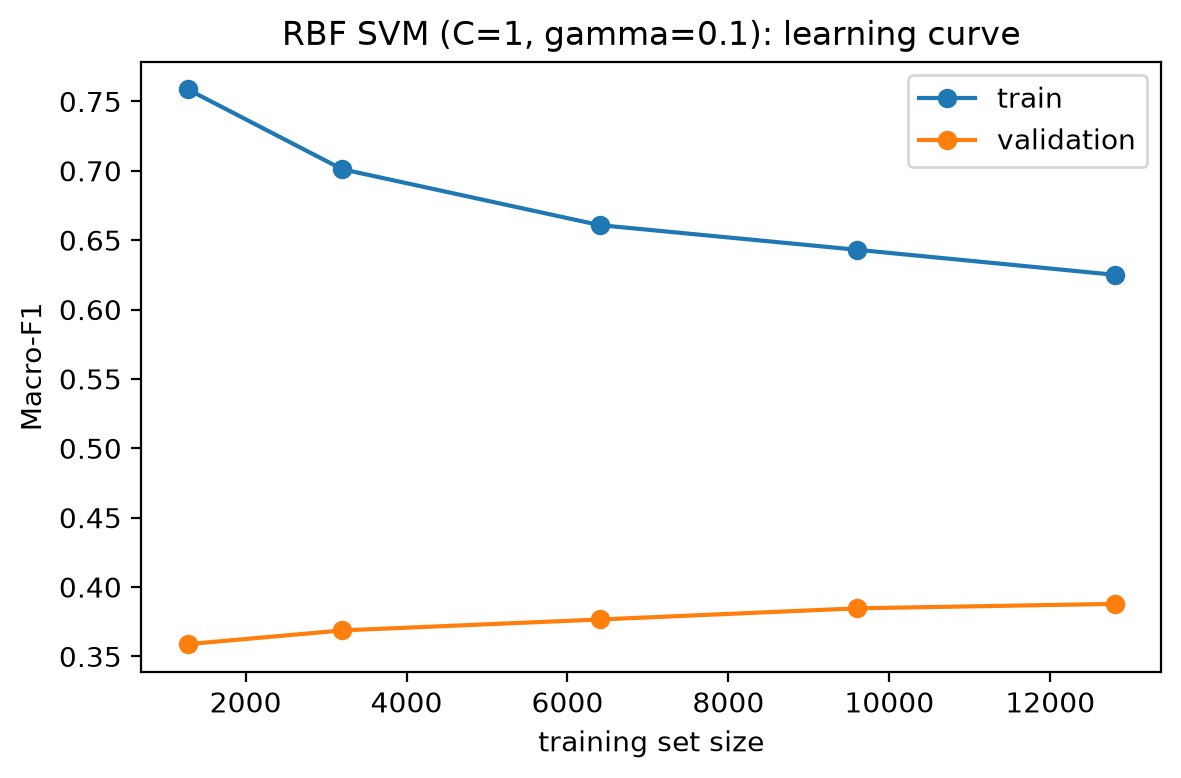
\includegraphics[width=\columnwidth]{figures/svm_learning_curve.png}
\caption{RBF SVM ($C=1$, $\gamma=0.1$) learning curve. Validation performance is still rising at the largest training size.}
\label{fig:svm-learning}
\end{figure}

Tuning settles on $C=0.3$ for linear (matching the plateau exactly) and $C=10$, $\gamma=0.03$ for RBF. On the held out test set, this produces the most striking result of the study so far: Linear SVM reaches 0.461 accuracy but only \textbf{0.351 Macro F1} and 0.365 balanced accuracy, while RBF SVM reaches nearly identical accuracy (0.464) but \textbf{0.409 Macro F1} and 0.396 balanced accuracy, a gap Accuracy alone completely hides. The reason is structural: the linear kernel achieves \textbf{0.000 precision, recall, and F1 on class 1}, never predicting it at all (655 of 714 true class 1 rows are assigned to class 2), while RBF raises class 1 recall to 0.217. This result is consistent with the hypothesis that a linear boundary struggles to separate an extreme class from a smoothly overlapping neighbor in a way a nonlinear kernel can \cite{cortes1995}. RBF also achieves the best class 5 recall (0.335) of any model evaluated so far, though 70\% of its class 5 errors still land in class 4. Linear SVM shows a similar concentration (78\% of its 136 class 5 errors land in class 4), consistent with the pattern already observed in the Decision Tree and kNN.

RBF costs more than linear in both directions (fit 9.92s vs.\ 6.10s, predict 2{,}704ms vs.\ 1{,}171ms), but its Macro F1 and balanced accuracy gains justify that cost. Both kernels are far more expensive than either prior algorithm, with linear SVM's predict time alone roughly 585x the Decision Tree's, making SVM the most computationally expensive model family in this study.

\subsection{Neural Networks}

Both implementations use \texttt{solver='sgd'}, \texttt{momentum=0}, no Nesterov acceleration, and no adaptive optimizer, per the assignment constraint. A single hidden layer is used throughout. Its width is the shared model complexity axis and is matched between implementations for a fair capacity comparison.

\subsubsection{scikit-learn MLP}

A learning rate sanity check (0.001, 0.01, 0.1) at a fixed starting width selects lr=0.01 (CV Macro F1 $0.435 \pm 0.011$, versus 0.406 for lr=0.001, too slow to converge without momentum, and 0.425 for lr=0.1, slightly worse and noisier). Regularization ($\alpha=10^{-4}$) and batch size (200) are stated explicitly rather than left as silent defaults. At this learning rate, a 32 unit baseline shows a training and validation gap of only 0.029 (0.464 vs.\ 0.435), far smaller than any other algorithm's baseline gap, suggesting this network is not prone to the severe overfitting seen elsewhere on this dataset.

Fig.~\ref{fig:nn-sk-complexity} sweeps hidden layer width from 2 to 128: validation Macro F1 peaks early, at width 8 (0.443), then gently declines and plateaus near 0.435 to 0.438 as training Macro F1 keeps climbing to 0.488, a much gentler overfitting curve than the Decision Tree's or RBF SVM's. That the optimum is a narrow 8 unit layer is consistent with EDA's finding that only a handful of features carry most of the separating signal. The learning curve (Fig.~\ref{fig:nn-sk-learning}) shows a healthy convergence pattern: training Macro F1 falls slightly (0.487 $\to$ 0.466) while validation rises (0.405 $\to$ 0.435), the gap nearly closing by the full training set.

\begin{figure}[htbp]
\centering
\begin{minipage}{0.49\columnwidth}
\centering
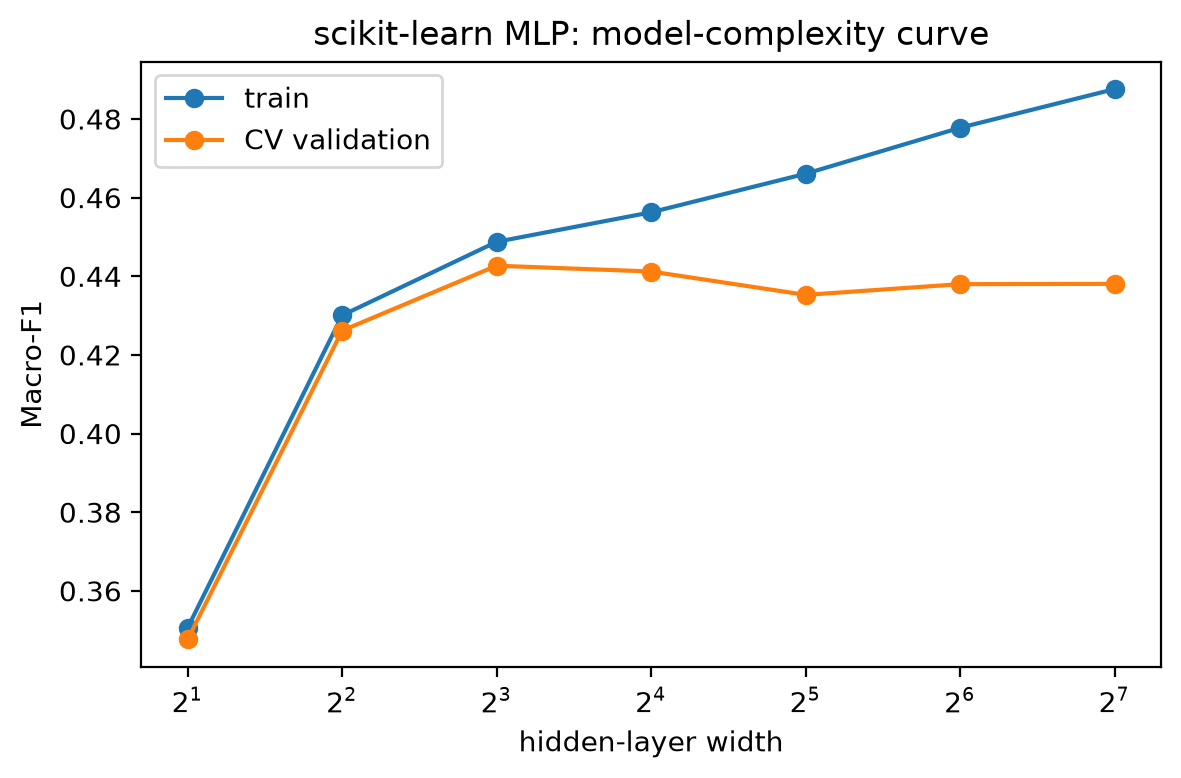
\includegraphics[width=\textwidth]{figures/nn_sklearn_complexity_curve.png}
\end{minipage}
\hfill
\begin{minipage}{0.49\columnwidth}
\centering
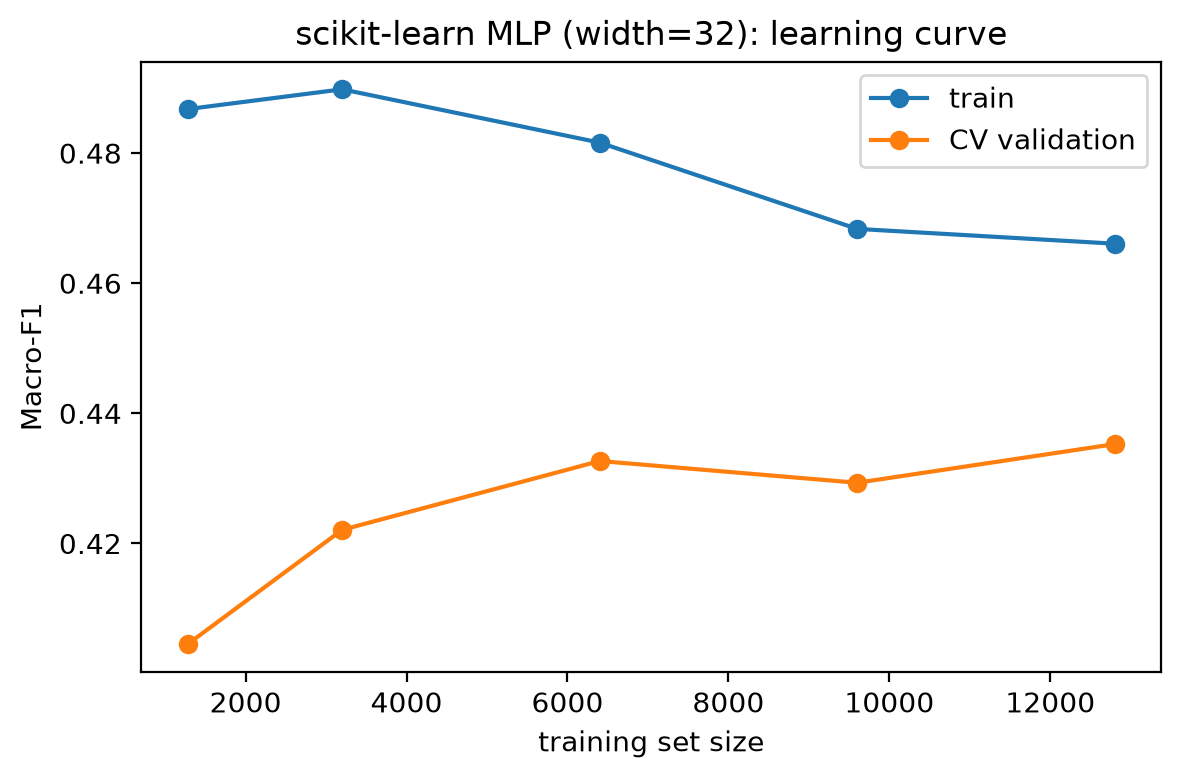
\includegraphics[width=\textwidth]{figures/nn_sklearn_learning_curve.png}
\end{minipage}
\caption{scikit-learn MLP model complexity curve (left, Macro F1 vs.\ hidden layer width, peaking at width 8) and learning curve at width 32 (right). Training and validation scores converge as data grows.}
\label{fig:nn-sk-complexity}
\label{fig:nn-sk-learning}
\end{figure}

Tuning confirms width 8. On the held out test set this is the \textbf{best result of the study so far}: 0.467 accuracy, \textbf{0.426 Macro F1}, and \textbf{0.410 balanced accuracy}, edging out the Decision Tree (0.421/0.401), kNN (0.410/0.386), and both SVM kernels (0.351/0.365 linear, 0.409/0.396 RBF) on the metrics that matter most for this imbalanced problem. Fit time is 1.72s and predict time 2.5ms, far cheaper than either SVM kernel and comparable to the Decision Tree's predict time, despite the higher score. This is currently the best accuracy for cost trade off in the study.

The epoch curve (Fig.~\ref{fig:nn-sk-epoch}) at the final architecture shows training loss decreasing smoothly across all 150 epochs with no instability, while validation Macro F1 is still rising at the final epoch (0.408). No improve then degrade pattern appears that would motivate early stopping, and no oscillation appears either, indicating lr=0.01 was a stable choice for plain SGD.

\begin{figure}[htbp]
\centering
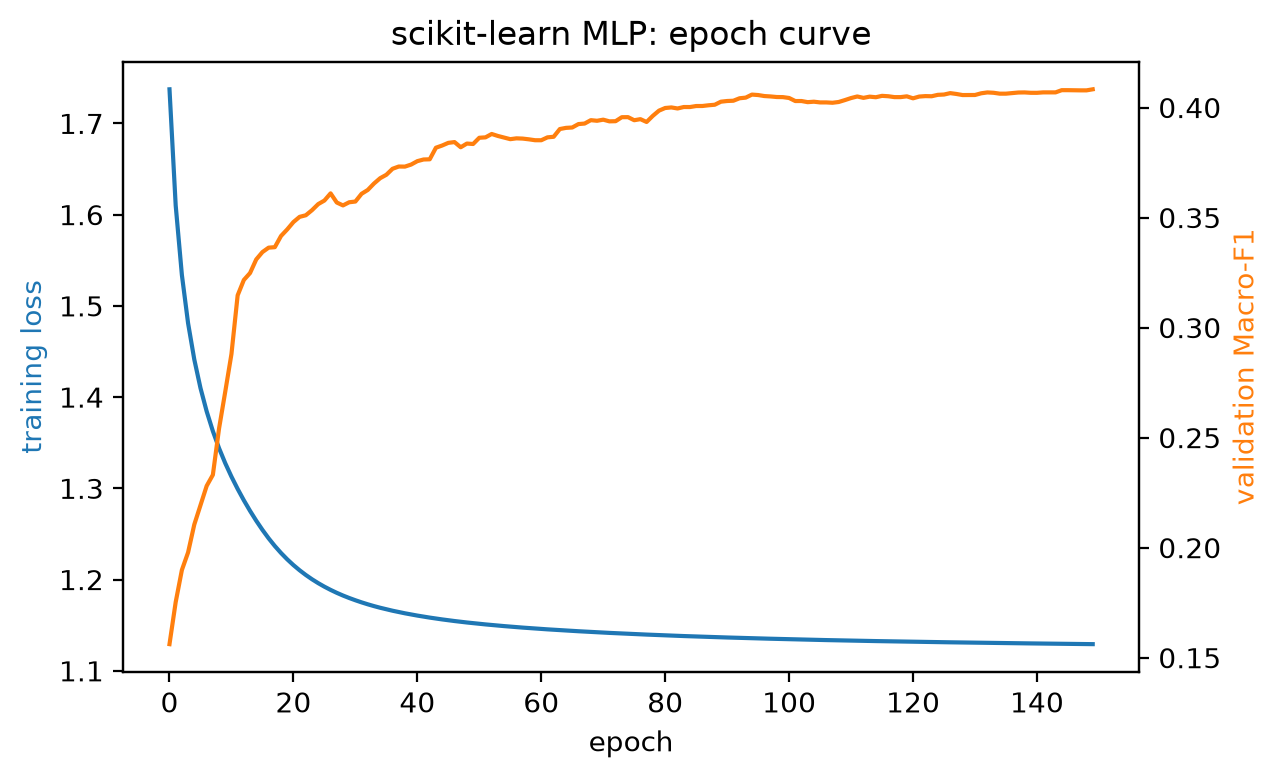
\includegraphics[width=\columnwidth]{figures/nn_sklearn_epoch_curve.png}
\caption{scikit-learn MLP epoch curve (final architecture). Training loss decreases smoothly. Validation Macro F1 is still rising at epoch 150.}
\label{fig:nn-sk-epoch}
\end{figure}

The class 3 recall (0.450) and class 5 recall (0.346) are the best achieved so far in this study, indicating that this network separates the middle and the rarest classes more evenly than the previous three algorithms. However, the class 4 and 5 boundary still remains the main source of mistakes: 108 of class 5's 125 mistakes (86\%, the highest concentration so far) land in class 4, consistent with the \texttt{BMI} plateau prediction.

\subsubsection{PyTorch MLP}

Manual PyTorch training loops take orders of magnitude more time per fit than scikit-learn's compiled implementation. Similar to the justification made earlier for SVM, this notebook tunes against a single 80/20 train/validation split rather than 5-fold CV, using the same grids for width and learning rate as the scikit-learn notebook for a fair comparison. The held out test set is accessed exactly once.

A sanity check of the learning rate right away reveals the first difference in the implementation: lr=0.1 wins (val Macro F1 0.435), a full \textbf{10x higher} than lr=0.01 (0.414 for lr=0.01, and lr=0.001 severely underfits at 0.270). The same constraint on both implementations does not imply the same optimal learning rate, probably due to different default weight initialization schemes and absence of sklearn's internal heuristics in the from scratch loop.

Fig.~\ref{fig:nn-pt-complexity} shows width sweep at lr=0.1: validation Macro F1 peaks at width \textbf{64} (0.440), an 8x difference from the scikit-learn's width 8 optimum on the same data and the same architecture family, another concrete implementation difference, although the single split protocol in this notebook introduces more noise into the validation scores than scikit-learn's CV. The learning curve (Fig.~\ref{fig:nn-pt-learning}) is correspondingly noisier than scikit-learn's, a natural price for the same protocol choice.

\begin{figure}[htbp]
\centering
\begin{minipage}{0.49\columnwidth}
\centering
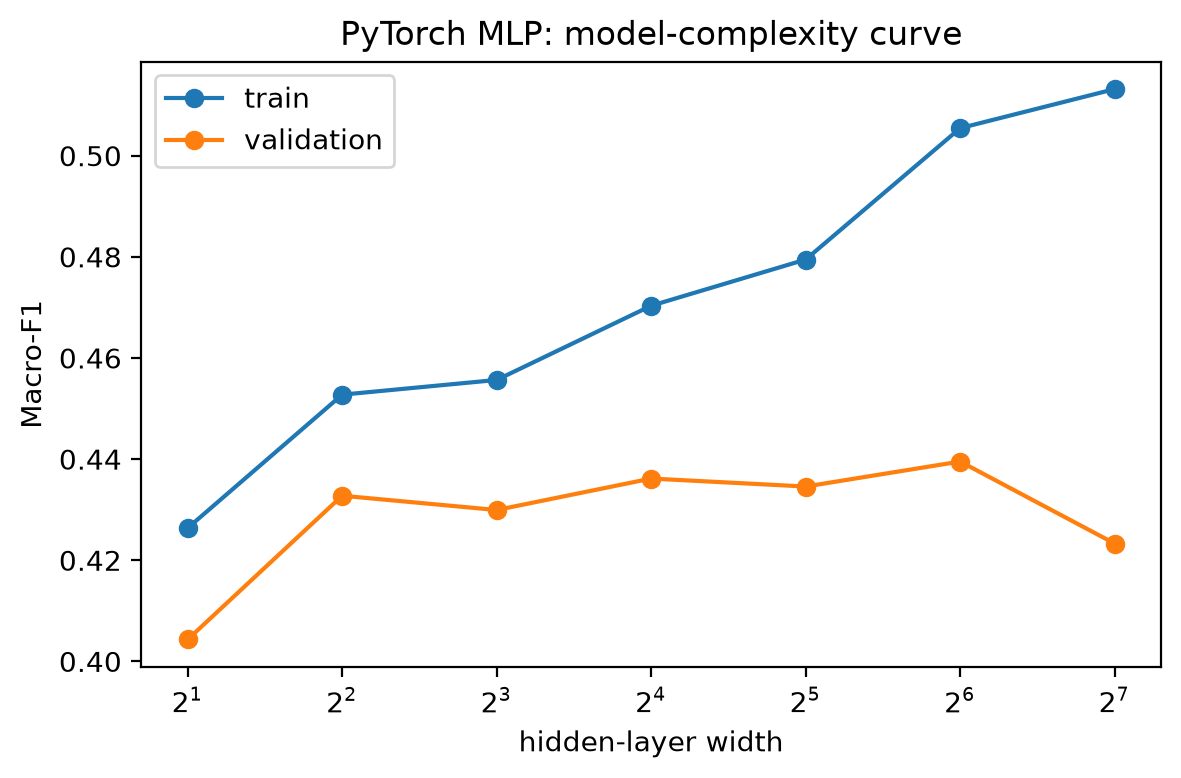
\includegraphics[width=\textwidth]{figures/nn_pytorch_complexity_curve.png}
\end{minipage}
\hfill
\begin{minipage}{0.49\columnwidth}
\centering
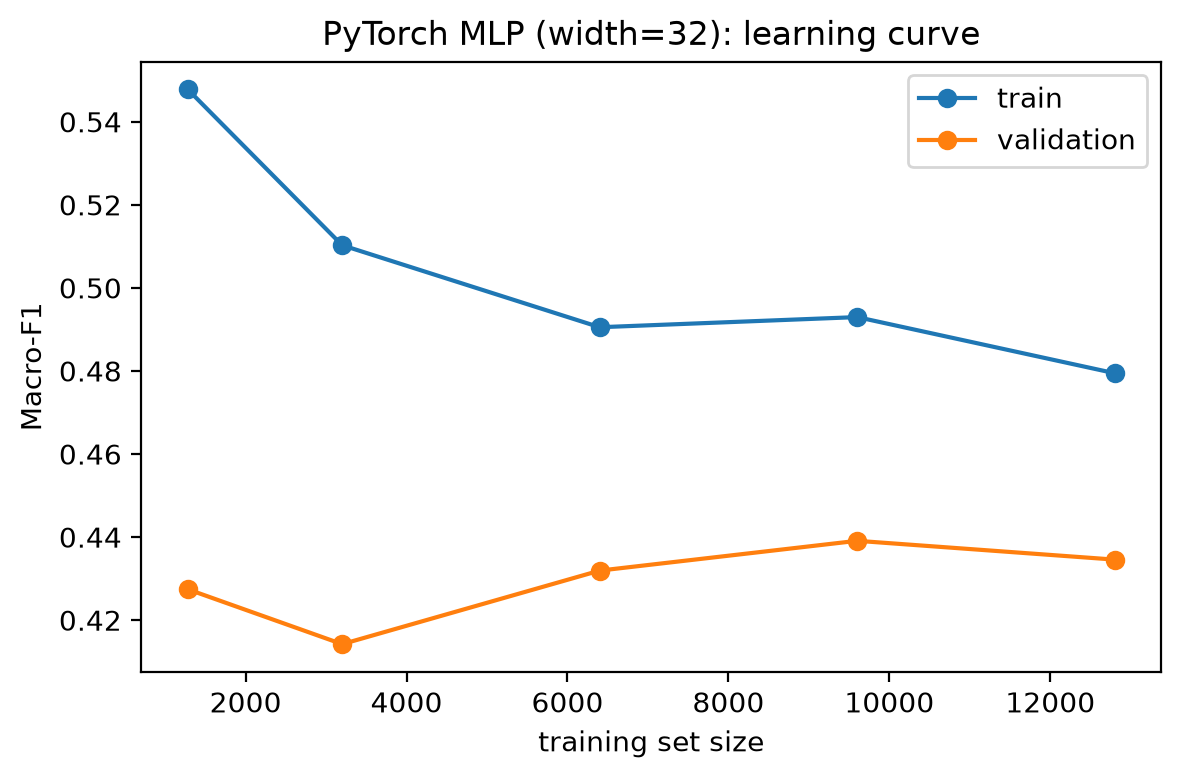
\includegraphics[width=\textwidth]{figures/nn_pytorch_learning_curve.png}
\end{minipage}
\caption{PyTorch MLP model complexity curve (left, Macro F1 vs.\ hidden layer width, peaking at width 64) and learning curve at width 32 (right), measured on a single validation split.}
\label{fig:nn-pt-complexity}
\label{fig:nn-pt-learning}
\end{figure}

Tuning confirms the width 64. On the held out test set, this produces the \textbf{best result of the whole study}: 0.463 accuracy, \textbf{0.444 Macro F1}, and \textbf{0.428 balanced accuracy}, beating the scikit-learn MLP (0.426/0.410), Decision Tree (0.421/0.401), kNN (0.410/0.386), and both SVM kernels. Fit time is 3.10s, almost twice scikit-learn's 1.72s, as expected, reflecting both wider architecture and overhead of the hand-written training loop. Predict time (2.1ms) is essentially identical to scikit-learn's.

As the best performing configuration in the study, this model's confusion matrix and per class precision, recall, and F1 are fully reported below. Table~\ref{tab:pytorch-confusion} shows the confusion matrix, and Table~\ref{tab:pytorch-perclass} the per class breakdown.

\begin{table}[htbp]
\caption{PyTorch MLP confusion matrix on the held out test set}
\label{tab:pytorch-confusion}
\centering
\small
\begin{tabular}{lrrrrr}
\toprule
 & \textbf{P1} & \textbf{P2} & \textbf{P3} & \textbf{P4} & \textbf{P5} \\
\midrule
True 1 & 273 & 352 &  82 &   7 &   0 \\
True 2 & 241 & 779 & 356 &  24 &   4 \\
True 3 &  77 & 455 & 550 &  99 &  12 \\
True 4 &   7 &  62 & 202 & 172 &  55 \\
True 5 &   0 &   4 &  26 &  85 &  76 \\
\bottomrule
\end{tabular}
\end{table}

\begin{table}[htbp]
\caption{PyTorch MLP per class precision, recall, and F1}
\label{tab:pytorch-perclass}
\centering
\small
\begin{tabular}{lrrrr}
\toprule
\textbf{Class} & \textbf{Prec.} & \textbf{Recall} & \textbf{F1} & \textbf{Support} \\
\midrule
1 & 0.457 & 0.382 & 0.416 & 714 \\
2 & 0.472 & 0.555 & 0.510 & 1404 \\
3 & 0.452 & 0.461 & 0.457 & 1193 \\
4 & 0.444 & 0.345 & 0.389 & 498 \\
5 & 0.517 & 0.398 & 0.450 & 191 \\
\bottomrule
\end{tabular}
\end{table}

The precision is comparatively flat across classes (0.444 to 0.517), unlike Linear SVM's complete collapse on class 1, indicating that this model does not systematically overpredict any particular class. Class 5 has the highest precision (0.517) despite being the rarest class, indicating that when the model predicts class 5 it is usually correct, although it recovers only 39.8\% of class 5 samples.

\begin{figure}[htbp]
\centering
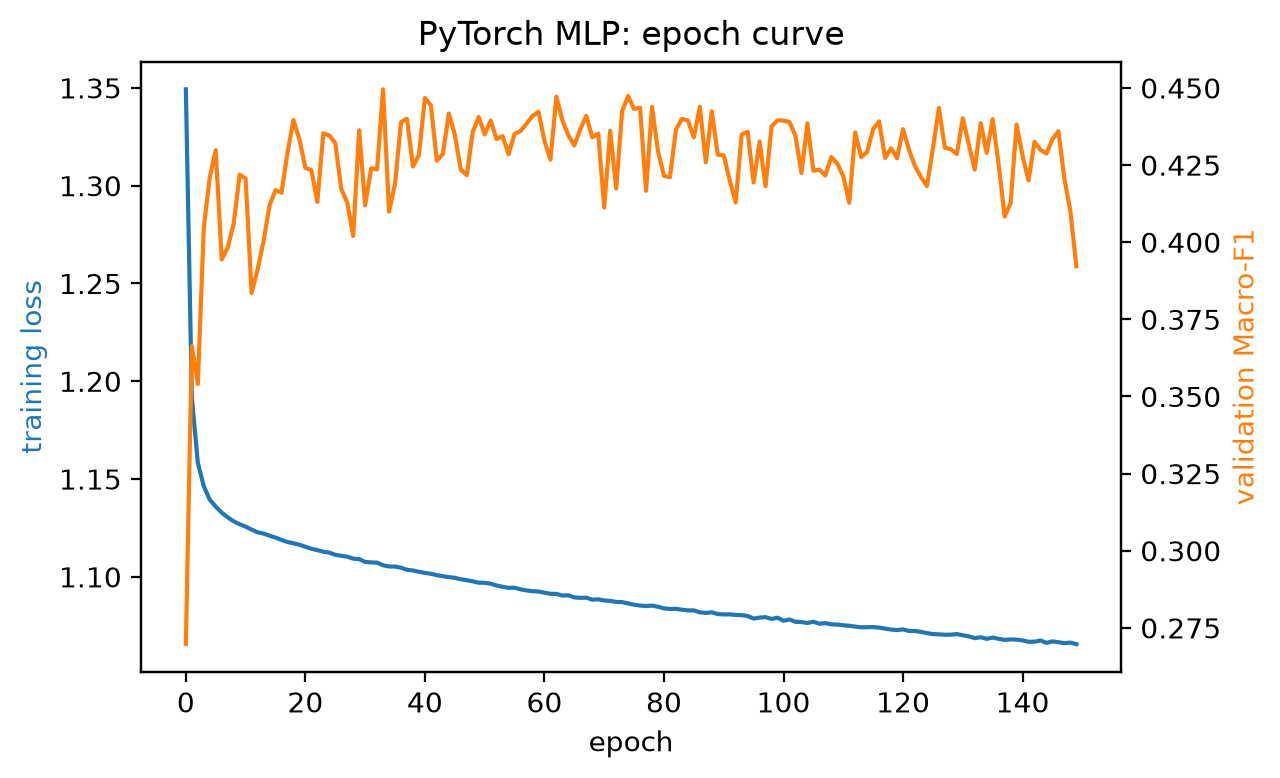
\includegraphics[width=\columnwidth]{figures/nn_pytorch_epoch_curve.png}
\caption{PyTorch MLP epoch curve (final architecture). Validation Macro F1 peaks at epoch 33 (0.450) then degrades to 0.392 by epoch 150, unlike scikit-learn's still rising curve.}
\label{fig:nn-pt-epoch}
\end{figure}

The epoch curve (Fig.~\ref{fig:nn-pt-epoch}) highlights the most significant difference in terms of implementation, with validation Macro F1 peaking at epoch 33 (0.450) and \textbf{degrading} to 0.392 by epoch 150, while training loss continues to drop smoothly. This is exactly the improve then degrade phenomenon that the assignment asked to detect, and scikit-learn's MLP showed no signs of degradation. One possible explanation is the higher learning rate: high enough to arrive at a good solution quickly, but lacking momentum or an adaptive step, continued training may move away from this optimum. No isolation experiment varying solely the learning rate was run to validate this cause of degradation. The validation curve suggests that early stopping is a plausible next step for the PyTorch implementation, while its effect on the held out performance has not been investigated, and no degradation was seen for scikit-learn's implementation.

This model is the best in terms of class 1 recall (0.382) and class 5 recall (0.398) of all model configurations. The class 4 and 5 boundary remains dominant: 85 of class 5's 115 errors (74\%) are misclassified as class 4. For all six models that were evaluated, this concentration is consistently between 65\% and 86\% regardless of algorithm family, the most consistent pattern of errors in this study.

\subsubsection{scikit-learn vs.\ PyTorch}

Both implementations use identical constraints (SGD, momentum=0, no Nesterov or adaptive optimizer, $\alpha$/weight\_decay=$10^{-4}$, batch size 200) yet diverge substantially in practice. scikit-learn converges reliably at a low learning rate (0.01) with a narrow 8 unit hidden layer and shows no instability even after 150 epochs. PyTorch requires a 10x higher learning rate (0.1) and a much wider 64 unit layer to reach its best score, and that score is only achievable with early stopping, since continued training visibly degrades validation performance past epoch 33. In other words, the same optimizer constraint produced a \textbf{stable but slightly weaker} implementation in scikit-learn and a \textbf{less stable but ultimately stronger} implementation in PyTorch (0.444 vs.\ 0.426 Macro F1) once tuned carefully. This reflects a tunability trade off: scikit-learn's implementation is more forgiving of hyperparameter and epoch budget choices, while PyTorch's implementation rewards more careful tuning with a higher ceiling in this experiment. Runtime favors scikit-learn slightly (1.72s vs.\ 3.10s fit, near identical predict times), though both remain far cheaper than either SVM kernel.

\section{Discussion}

\subsection{Cross Model Comparison}

Table~\ref{tab:final-comparison} summarizes the final performance and runtime for all six model configurations. There is no one model that wins all metrics: the PyTorch MLP model has the best Macro F1 and balanced accuracy, the scikit-learn MLP has the best accuracy, and the Decision Tree is significantly cheaper than everything else.

\begin{table}[htbp]
\caption{Final comparison across all model configurations}
\label{tab:final-comparison}
\centering
\small
\begin{tabular}{lrrrrr}
\toprule
\textbf{Model} & \textbf{Acc.} & \textbf{M F1} & \textbf{B.Acc.} & \textbf{Fit(s)} & \textbf{Pred.(ms)} \\
\midrule
Decision Tree     & 0.443 & 0.421 & 0.401 & 0.024 &    2.0 \\
kNN ($k$=21)      & 0.444 & 0.410 & 0.386 & 0.005 &   57.6 \\
Linear SVM        & 0.461 & 0.351 & 0.365 & 6.10  & 1170.6 \\
RBF SVM           & 0.464 & 0.409 & 0.396 & 9.92  & 2703.5 \\
MLP (sklearn)     & 0.467 & 0.426 & 0.410 & 1.72  &    2.5 \\
MLP (PyTorch)     & 0.463 & \textbf{0.444} & \textbf{0.428} & 3.10  &    2.1 \\
\bottomrule
\end{tabular}
\end{table}

Accuracy alone provides an overly simplified picture: all six numbers fall into a very narrow 0.024 range of values. On the contrary, Macro F1 spreads the six models across 0.093 range, totally reordering them, with Linear SVM dropping from second highest Accuracy to last place, showing why Accuracy alone is an inadequate metric for an imbalanced multiclass problem \cite{he2009}.

\subsection{Hypothesis Revisited}

The hypothesis is \textbf{partially supported}. Its first part regarding extreme classes held true in full: the Decision Tree (class 1 recall 0.319, class 5 recall 0.330) easily matched or beat the Linear SVM (class 1 recall \textbf{0.000}, class 5 recall 0.288) at both extremes, just as predicted. The linear method structurally cannot output class 1 at all, while tree's threshold splits deal well with it. The second part of the hypothesis, that either RBF SVM or MLP would outperform the Decision Tree on the harder adjacent pairs (2 vs.\ 3, 3 vs.\ 4), held true only for the MLPs and for class 3: both networks outperformed the tree's class 3 F1 (0.433) by a considerable margin (0.457 each), consistent with a smooth, overlapped boundary favoring a non-linear model. This was not the case for class 4, where tree's F1 (0.401) was comparable with or superior to that of all other models including RBF SVM (0.361), nor RBF SVM outperformed the tree on class 3 (F1 0.443 vs.\ 0.433, a negligible margin) or class 4 at all. The second prediction, persistent confusion between classes 4 and 5, proved clearly correct and was the most consistent pattern of errors in the study: 65\% to 86\% of all errors of every model for class 5 ended up in class 4, in all six configurations. This pattern is consistent with \texttt{BMI}'s very similar class conditional means for classes 4 and 5, although the experiments don't prove the individual contribution of \texttt{BMI} to the results.

\subsection{Performance, Runtime, and Class Level Behavior}

The PyTorch MLP configuration is the best in terms of Macro F1 and balanced accuracy, and it also has 2.1ms predict time matching the Decision Tree's. The RBF SVM becomes less attractive given the observed trade off of performance and runtime in this experiment: both MLPs beat its Macro F1, while being roughly 1,000x cheaper to predict (2.1ms to 2.5ms vs.\ 2{,}703.5ms). Within SVM family, RBF version's increased cost (fit 9.92s vs.\ 6.10s) corresponds to increased capabilities, saving class 1 from complete failure. Class level performance pattern is consistent through the whole study: class 2 (the biggest class) is easiest for all models, classes 1 and 5 (smallest, most extreme classes) are hardest for all models except the two MLPs, and the class 4 and 5 boundary is the main source of errors for all model configurations.

\subsection{Limitations and Improvement}

The most obvious limitation is specific and evidence-based, not generic: the final PyTorch MLP model was trained using a fixed epoch budget of 100 epochs selected prior to having the epoch curve (Fig.~\ref{fig:nn-pt-epoch}) available, which showed validation Macro F1 peaking at epoch 33 (0.450) and degrading to 0.392 by epoch 150 using the same architecture and learning rate. Thus, epoch number was not considered a tunable hyperparameter for this model. The obvious improvement is retraining the final model with early stopping, stopping the fitting process once validation Macro F1 fails to improve for a fixed number of epochs. The validation curve suggests that early stopping is a reasonable follow-up, although its effect on held-out performance remains uninvestigated.

\section{Conclusion}

For six model configurations representing four algorithm families, no single model dominates every metric, but a consistent pattern emerges: nonlinear or threshold based decision boundaries (Decision Tree, both MLPs) cope with the dataset's class structure much better than the purely linear one, and choice of the metric matters. The hypothesis was partially supported. It was correct about the Decision Tree matching the linear methods at the extremes and about persistent confusion between classes 4 and 5, which is consistent with, but cannot be attributed to, \texttt{BMI}'s limited separation between those two classes. It was too specific in assigning the middle class advantage to RBF SVM, which is shown by the evidence to be due to the two MLPs. Assuming class 5 is the positive class in a one versus rest scenario, the major error is a Type II error: respondents with Poor self reported health (class 5) are predicted as Fair (class 4) much more often than anything else, for every algorithm, making a deployed model built on this data underestimate rather than overestimate health severity, which is the more consequential direction of the error for a health screening application. Class imbalance was relevant to the interpretation in this study, most prominently in the split between competitive Accuracy and near worst Macro F1 of Linear SVM. The most obvious next step is to retrain the PyTorch MLP model using early stopping, and test class weighting for class 5, since the best model achieved only 39.8\% of the true class 5 instances.


\section*{AI Use Statement}

I used Claude as an assistance tool throughout the assignment. However, Claude did not do the work for me. The analysis, decisions, experiment structure and experiment, results, and report are my own. I have chatted back and forth with Claude to plan and discuss directions to proceed. When writing code, I used Claude to generate code chunks for specific functions which is based on strict requirements given by me. I have reviewed, verified, and understand all assisted content. 


\begin{thebibliography}{3}
\bibitem{teboul2021} A. Teboul, ``Diabetes Health Indicators Dataset,'' Kaggle, 2021. [Online]. Available: https://www.kaggle.com/datasets/alexteboul/diabetes-health-indicators-dataset
\bibitem{cortes1995} C. Cortes and V. Vapnik, ``Support-vector networks,'' Machine Learning, vol. 20, no. 3, pp. 273 to 297, 1995.
\bibitem{he2009} H. He and E. A. Garcia, ``Learning from imbalanced data,'' IEEE Transactions on Knowledge and Data Engineering, vol. 21, no. 9, pp. 1263 to 1284, 2009.
\end{thebibliography}

\end{document}
